% https://tex.stackexchange.com/a/452487/173708
\documentclass[tikz,border=3.14mm]{standalone}
\usetikzlibrary{shapes.arrows,arrows.meta}

\begin{document}
	
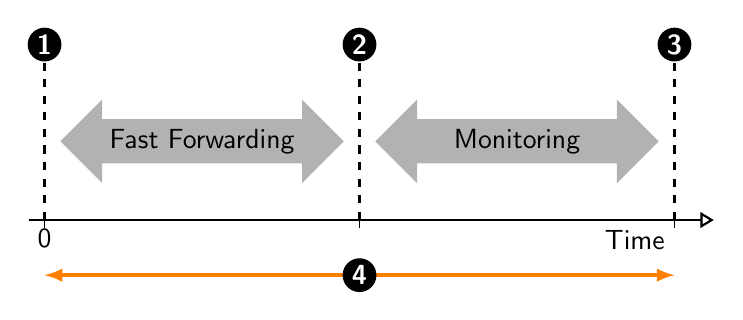
\begin{tikzpicture}[font=\sffamily, 
	bullet/.style={fill=black, 
		circle, 
		text=white, 
		font=\sffamily\bfseries, 
		inner sep=1.2pt}]
	
	\draw[thick,-{Triangle[open]}] (-0.2,0) -- (8.5,0);
	\foreach \X in {1,2,3} {
		\draw ({(\X-1)*4},0.1) -- ({(\X-1)*4},-0.1);
		\draw[thick,dashed] ({(\X-1)*4},0) -- ++(0,2)
		node[above,bullet]{\X};}
	\node [double arrow, fill=gray!60,minimum height=3.6cm] at (2,1) {Fast Forwarding};
	\node [double arrow, fill=gray!60,minimum height=3.6cm] at (6,1) {Monitoring};
	\draw[orange,very thick,latex-latex] (0,-0.7) -- (8,-0.7) node[midway,bullet]{4};
	\node[anchor=north] at (0,0) {0};
	\node[anchor=north east] at (8,0) {Time};
\end{tikzpicture}
\end{document}